\chapter{Background}


%%%%%%%%%%%%%%%%%%%%%%%%%%%%%%%%
%         Cosmic-ray
%%%%%%%%%%%%%%%%%%%%%%%%%%%%%%%%
\section{Cosmic-ray}

This section consists of historical discovery, from the origin
on this field of study until the latest impactful experiment.
Not only historical content, it also contains the physical
explaination with phenomenon that involving the CR reserch.

\subsection{History}
In 1909, the famous experiment that pioneer the study of CR has been
led by Theodor Wolf who take conduct the experiment of 
altitude variation by taking the apparatus to measure 
the rate of ionization from the ground to the top of 
the Eiffle Tower in Paris (\cite{gray1949cosmic}).
The result shown that there the ionizaiton rate was slightly
increase when the altitude is higher which gives the clues
that the origin of cosmic-rays was came from the outer space
rather than Earth's inner shell.

However, the experiment of measuring the affect of altitude
variation with a tiny altitude scale comparing to the Earth's
atmosphere would not enough to consolidate the theory.
In the same year, the ballon with a similar instrument has
been released up to 1.3 kilometers by Karl Bergwitz to put 
more weight on the first experiment. They found that the 
ionization has increased by a quater comparing to ground level 
(\cite{de2014atmospheric}).
Three years later, suicidal investigation was conducted by 
an Australian gentleman who brought the detector and himself
to fly with the balloon.
His name is Victor Hess, people might have no doubt why this
name went so famous because he risk his life with the experiment 
and he was flying over 5 kilometers above the ground (\cite{hess1912beobachtungen}).
Definitely, the result is strongly significant and impactful
to the astrophysical research community. Risking life  
In 1914, Werner Kolhörster repeated the balloon experiment 
with higher altitude which around 9 kilometers from the 
sea level and the ionizaiton rate still does increase when 
the ballon flown higher. This emphasize that the source of 
those ionizing ray came from Earth's upper atmosphere
or the outer space.

Not only the altitude variable that related to the 
intensity of the CRs, but the geographic location of the 
obvervation also does affect to the measurement.
The first experiment has done done John Clay who
sailed the ship across the ocean from Holland to Java
(\cite{Clay1927,Clay1928}). The result shows that
the further from equator, the higher CR intensity.
Another exploration for the geographic variation was 
done by John Compton in the following five years.
He basically sailed the ship from the Sydney (northern hemisphere)
to Vancouver (the southern hemisphere) for various season
during 1936 to 1937 back and forth (\cite{compton1937cosmic}).
The Figure \ref{fig:comptonship} demonstrates the 
latitude variation and the seasonality effects of the 
multiple trips from the experiment.

\begin{figure}[h!]
    \centering
    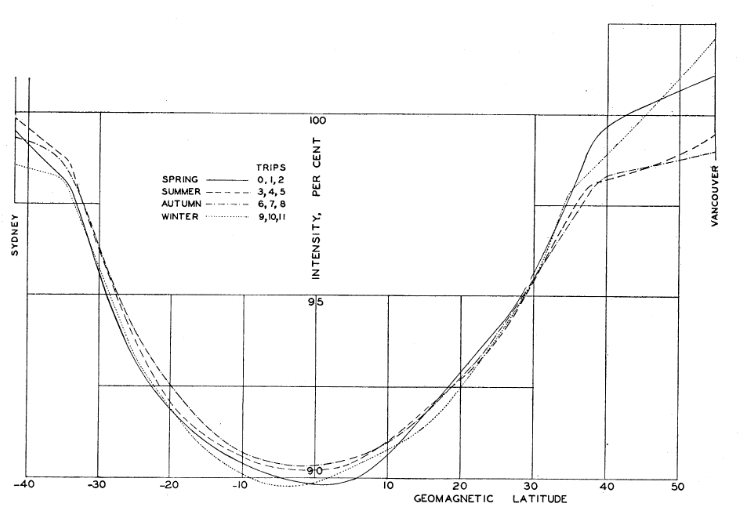
\includegraphics[width=\textwidth]{content/background/figures/compton_sail_1937.png}
    \caption{Latitude variation for various seasons (\cite{compton1937cosmic})}
    \label{fig:comptonship}
\end{figure}
	
The first interpretation study from the discovery has been
done by Carl Störmer. The explaination of the CR's altitude variation
came from the trajectory of CR particles due to geomagnetic field
(\cite{stormer1934critical}). In that period, the topic of 
geomagnetic field and the effects of CRs was quite famous.
Another impactful study of the CRs trajectory and the relevant
of Earth's magnetic field was conducted by Bruno Rossi
for predicting an asymmetry of the East-West distribution
of CR spectrum because the primary CRs does have a positive or
negative charge then the cyclic moving direction of the 
particle was induced by Lorentz force where the direction of 
the Earth's magnetic field could be identified to determine the
direction of the charged particles (\cite{rossi1941cosmic}).

The ground based detector is a great option for 
detecting the CRs where it include primary and secondary CRs.
However, investigating the primary CRs is a challenging topic
for ground based detector especially for low energy particles.
Another interesting option to inspect the asymmetry of 
East-West could be done by using space based detector 
that orbiting around the Earth's at some radius in the
higher altitude and definitely it would face a lower 
atmospheric density which consider to be an interesting 
choice to study the CRs with a lower effects of atmospheric
interaction.

In 2008, \textit{Fermi} Large Area Telescope (LAT)
has been launched to observed the $\gamma$-ray and the
lightweight lepton particles which basically are electron
and position. 

\subsection{Physical properties}
The physical properties


\subsection{$\gamma$-ray production}

\subsection{Earth's limb $\gamma$-ray production}

%%%%%%%%%%%%%%%%%%%%%%%%%%%%%%%%
%         Fermi-LAT
%%%%%%%%%%%%%%%%%%%%%%%%%%%%%%%%
\section{\textit{Fermi} Large Area Telescope (LAT)}

\subsection{Overview}

\subsection{Apparatus}

\subsection{Event reconstruction}




% \begin{figure}[h!]
%     \centering
%         \subfloat[Victor Hess in his balloon]{
%             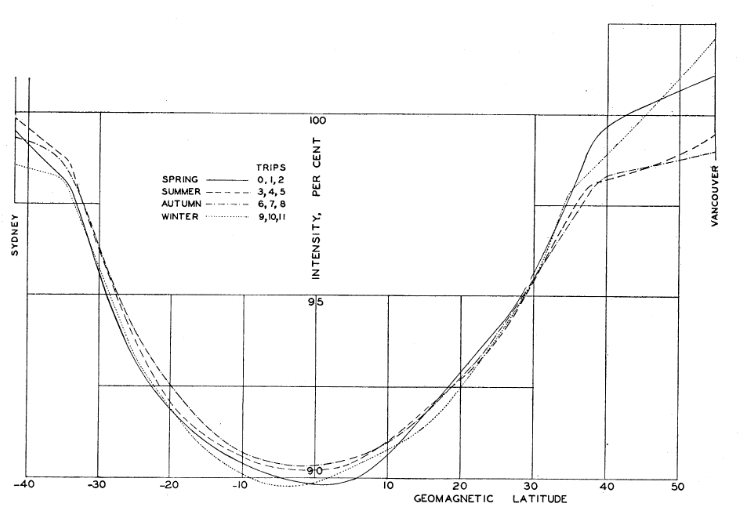
\includegraphics[width=0.45\textwidth]{content/background/figures/compton_sail_1937.png}
%             }
%         \hfill
%          \subfloat[The ion pairs rate vs the altitude (km) detected using ion chambers by Victor Hess (left) and Werner Kolh\"orster (right)]{
%             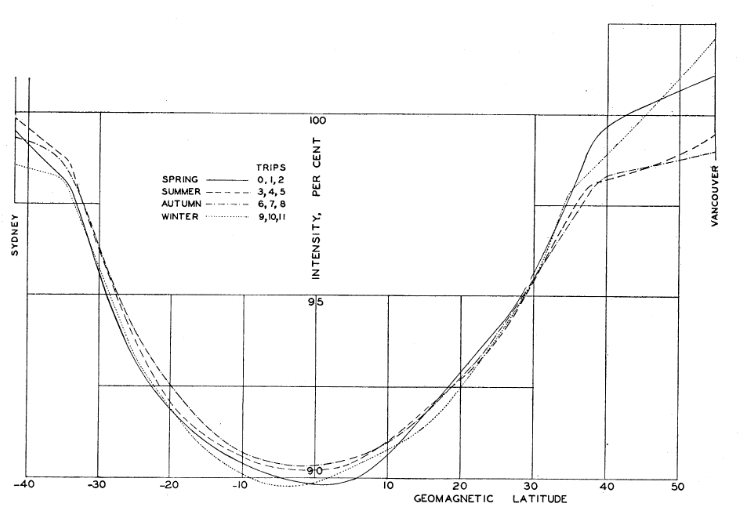
\includegraphics[width=0.45\textwidth]{content/background/figures/compton_sail_1937.png}
%             }
%         \caption[CR discovery experiment by Victor Hess in 1912 (a) and the confir- mation by Werner Kolh\"orster in 1914 (b).]{CR discovery experiment by Victor Hess in 1912 (a) and the confirmation by Werner Kolh\"orster in 1914 (b). }
%        \label{fig:comptonsail}
% \end{figure}